
\section{Разработка и реализация алгоритма защиты}
\label{sec:--1}

\subsection{Описание целей и способа защиты}
\label{subsec:--1}

В соответствии с заданием на курсовой проект, защита программы от
несанкционированного копирования осуществляется посредством
ограничения времени работы незарегистрированной программы. Данный
способ защиты обеспечивает возможность ознакомления пользователя с
программой без ее приобретения. Это позволяет предоставить
использование программы пользователям, которые не планируют ее
постоянно использовать, либо хотят принять решение о
целесообразности ее приобретения. Для снятия ограничения по
использованию программы следует произвести регистрацию программы с
помощью пароля. Знание пароля является свидетельством прав на
обладание программой и должно предоставляться правообладателем.

Защита программы должна контролировать наличие регистрации. При этом
программа должна регистрироваться однажды и не требовать ввода пароля
при каждом запуске.  В качестве механизма определения возможностей
пользователя при работе с программой выступает признак регистрации
программы, сохраняемый в реестре операционной системы. В качестве
признака выступает текстовая строка, содержащая ключевую фразу.

Признак регистрации проверяется при запуске. В случае отсутствия
регистрации проверяется срок использования незарегистрированной
программы. Если он не превышает установленного, программа запускается,
в противном случае предлагается зарегистрировать программу. До
регистрации программы доступ к полезным функциям программы
блокируется.

При регистрации создается соответствующий ключ реестра, в который
записывается строка регистрации.

Пароль защищается в коде программы регистрации применением встроенной
в Visual Studio хэш-функции.

\subsection{Описание алгоритма защиты}
\label{subsec:--2}

При запуске программы проверяется наличие записи в ключе реестра. Если
ключ не найден, либо его содержимое не совпадает с признаком
регистрации, то осуществляется проверка срока использования
программы. Для этого из файла считывается дата установки программы. К
полученной дате прибавляется срок использования незарегистрированной
программы, равный 5 дням. Полученная дата сравнивается с текущей. Если
рассчитанная дата меньше текущей, доступ к полезным функциям программы
блокируется и пользователю предлагается произвести регистрацию
посредством пароля.

Если пользователь желает пройти регистрацию, то запускается процедура
регистрации. Процедура регистрации включает правильность проверки
пароля пользователя. Если пароль верен, в ключ реестра записывается
строка-признак регистрации. При вводе неверного пароля выдается
соответствующее сообщение, и регистрация не проходит.  Если содержание
ключа реестра, используемого программой, соответствует установленному
признаку регистрации, то программа считается зарегистрированной и
запускается без проверки срока использования.

Блок-схема разработанного алгоритма приведена в
Приложении~А.

\subsection{Описание программной реализации алгоритма защиты}
\label{sec:--3}

Для реализации разработанного алгоритма защиты программы была
разработана программа, выполняющая генерацию псевдослучайной
последовательности со встроенной защитой от несанкционированного
копирования, а также программа установки, осуществляющая настройку
параметров защиты для основной программы. 

Для разработки программы использовалась интегрированная среда
разработки Visual Studio Express 2010. Для написания программы был
использован язык программирования Visual C++.  Функция регистрации
позволяет снять ограничения для легальных пользователей. Она включает
проверку пароля пользователя и, в случае ввода правильного пароля,
создает ключ реестра, содержащий признак регистрации. Данная функция
реализована в виде обработчика нажатия кнопки на главной форме
проекта (листинг~\ref{1.cpp}).

\begin{lstlisting}[caption = {Функция регистрации}, label = {1.cpp}]
private: System::Void button2_Click(System::Object^  sender, System::EventArgs^  e) {
 int pass = this->textBox1->Text->GetHashCode();
 int right_pass = 1364505728; 
 if(pass==right_pass)
 {
	  RegistryKey^ rk = nullptr;
	  rk = Registry::CurrentUser->OpenSubKey("GPSP",true);
	  if (rk==nullptr)
	  {
			 RegistryKey^ rk = Registry::CurrentUser->CreateSubKey("GPSP");
			 rk->SetValue("line","forza");
			 rk->Close();
	  }					
	  else
	  {
			 Registry::CurrentUser->DeleteSubKey("GPSP");
			 RegistryKey^ rk = Registry::CurrentUser->CreateSubKey("GPSP");
			 rk->SetValue("line","forza");
			 rk->Close();
	  }
	  this->groupBox1->Hide();
	  this->groupBox2->Show();
	  MessageBox::Show("Зарегистрировано");
 }
 else
 {
	 MessageBox::Show("Неправильный пароль");
 }

} 
\end{lstlisting}

Основная программа содержит функцию проверки наличия ключа реестра и
правильность значения, записанного в него. 

Данная функция вызывается при загрузке программы, при обработке
события \texttt{Form\_Load}. Если регистрация отсутствует, программа
проверяет, не превышен ли срок использования программы. Для этого из
файла созданного при установке программы считывается дата
установки. Сравнение дат, осуществляется с использованием методов
встроенного класса \texttt{DateTime} (листинг~\ref{2.cpp})~\cite{2}.

\begin{lstlisting}[caption = {Проверка признака регистрации}, label = {2.cpp}]
 bool reg = true;
 RegistryKey^ rk = nullptr;
 rk = Registry::CurrentUser->OpenSubKey("GPSP",true);
 if (rk==nullptr)
 {
	reg = false;
 }
 else
 {
	 String^ value = rk->GetValue("line")->ToString();
	 if(value!="forza") reg = false; 
 }
 DateTime^ dt = DateTime::Now;
 if(!reg)
 {
	 
	 StreamReader^ read_date = gcnew StreamReader("param");
	 DateTime^ start = Convert::ToDateTime(read_date->ReadLine()); 
	 if(DateTime::Compare(start->AddDays(5), dt->Date)<0)
	 {
		 MessageBox::Show("Срок использования незарегистрированной версии истек. Хотите зарегистрировать программу");
		 this->groupBox2->Hide();
	 }
	 else this->groupBox1->Hide();
 }
 else this->groupBox1->Hide(); 
\end{lstlisting}

Интерфейс основной полезной программы приведен на рисунке~\ref{fig:1}.

\begin{figure}[h!]
  \centering
  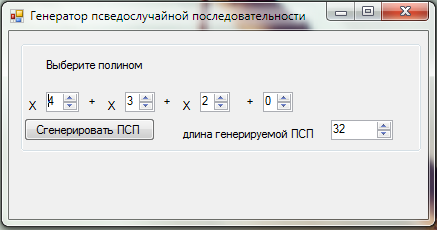
\includegraphics[]{interface}
  \caption{Интерфейс программы}
  \label{fig:1}
\end{figure}

Для проверки корректности работы защиты программы было осуществлено
изменение системной даты на 7 дней вперед. На рисунке~\ref{fig:2}
отображено сообщение об окончании периода использования
незарегистрированной программы.

\begin{figure}[h!]
  \centering
  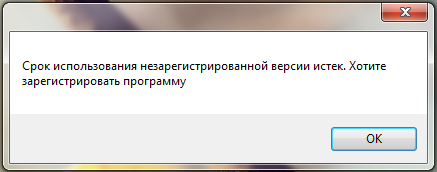
\includegraphics[]{register_message}
  \caption{Сообщение об окончании периода использования
    незарегистрированной программы}
  \label{fig:2}
\end{figure}

Блокирование полезных функций программы после окончания периода
использования незарегистрированной программы представлено на
рисунке~\ref{fig:3}.

\begin{figure}[h!]
  \centering
  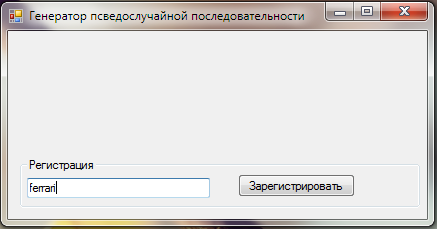
\includegraphics[]{register}
  \caption{Блокирование полезных функций после окончания периода
    использования незарегистрированной программы}
  \label{fig:3}
\end{figure}

Полный текст основной программы, а также программы установки приведен
в Приложении Б.

\section{Анализ стойкости использованного алгоритма защиты}
\label{sec:--4}

В ходе исследования выявляются сведения, которые могут быть
использованы нарушителем для проведения атак на защиту программы. На
данном этапе использовались следующие программные средства
анализа\cite{4}:

\vspace{-5mm}
\begin{itemize}
\item дизассемблер \textit{IDA}, позволяющий произвести статическое
  исследование дизассемблированного листинга программы;
\item утилита мониторинга \textit{ProcessMonitor}, осуществляющая
  контроль активности приложения при обращениях к ресурсам файловой
  системы, реестра и системным вызовам;
\item отладчик \textit{OllyDbg}, позволяющий произвести динамическое
  исследование логики работы программы.
\end{itemize}

\subsection{Анализ защиты с использованием дизассемблера}
\label{sec:--5}

Первым этапом исследования являлось дизассемблирование программы. В
результате анализа полученного кода выявлен механизм проверки
регистрации, представленный на рисунке~\ref{fig:4}.

\begin{figure}[h!]
  \centering
  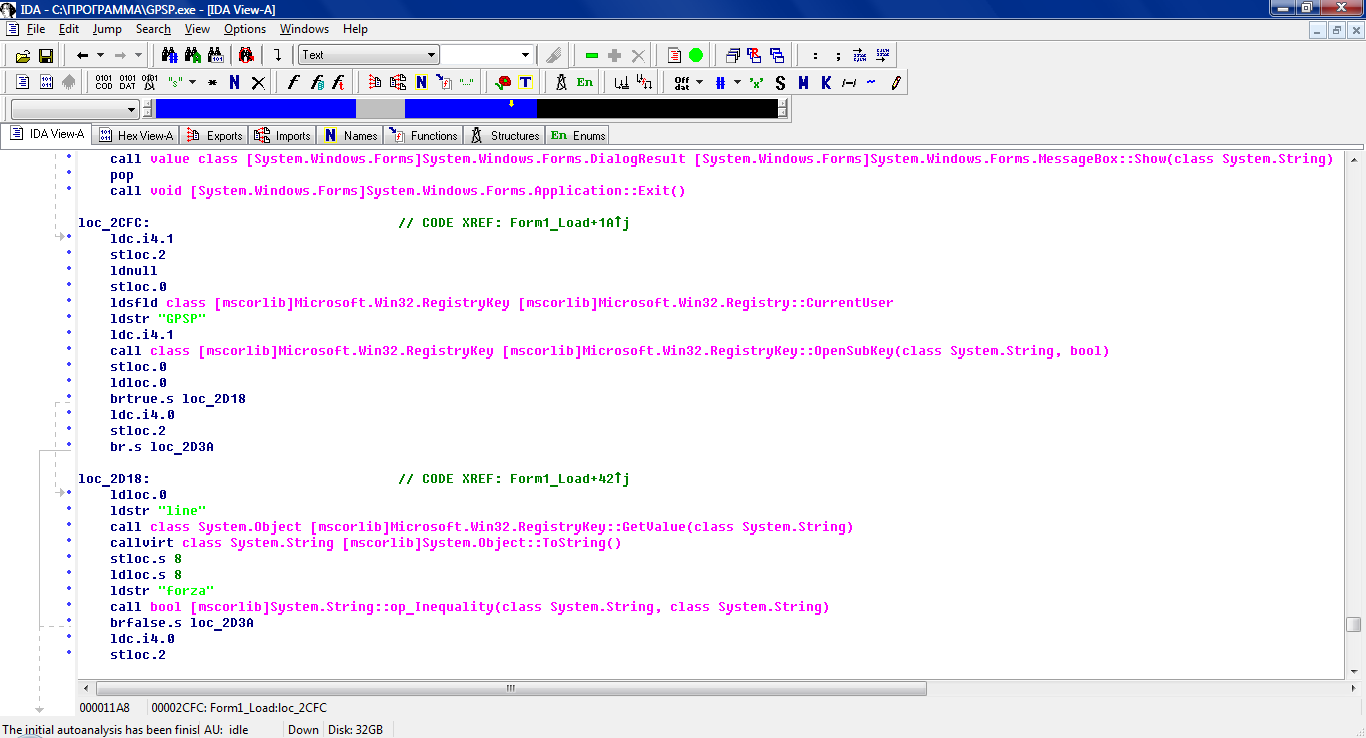
\includegraphics[width=\textwidth]{register_chech}
  \caption{Функция проверки регистрации программы}
  \label{fig:4}
\end{figure}

На данном рисунке отмечены функции считывания значения ключа реестра и
функция сравнения с признаком регистрации. Признак регистрации при
этом хранится в явном виде (строка). Данные сведения могут быть
использованы при создании признака регистрации несанкционированным
способом.

В обработчике кнопки регистрации были выявлены механизмы проверки
пароля пользователя и хэш от верного пароля, а также создания признака
регистрации в ключе реестра. Данные элементы отмечены на
рисунке~\ref{fig:5}.

\begin{figure}[h!]
  \centering
  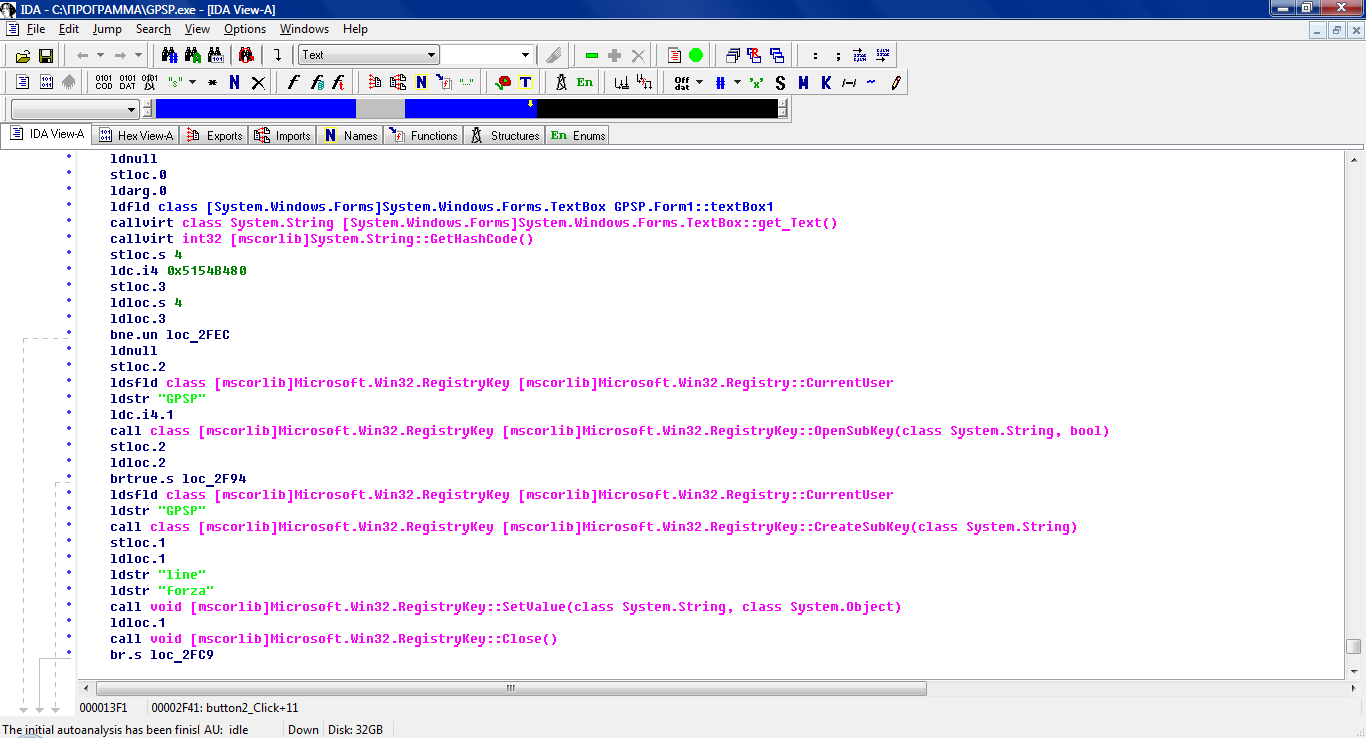
\includegraphics[width=\textwidth]{check_password}
  \caption{Проверка пароля пользователя при регистрации}
  \label{fig:5}
\end{figure}

Таким образом, атака на пароль затруднена, поскольку в программе
хранится лишь проверочное значение хэш, и наиболее эффективным
способом будет простой перебор всех возможных паролей.  

Также была исследована функция проверки срока использования
программы. Данная функция представлена на рисунке~\ref{fig:6}.

\begin{figure}[h!]
  \centering
  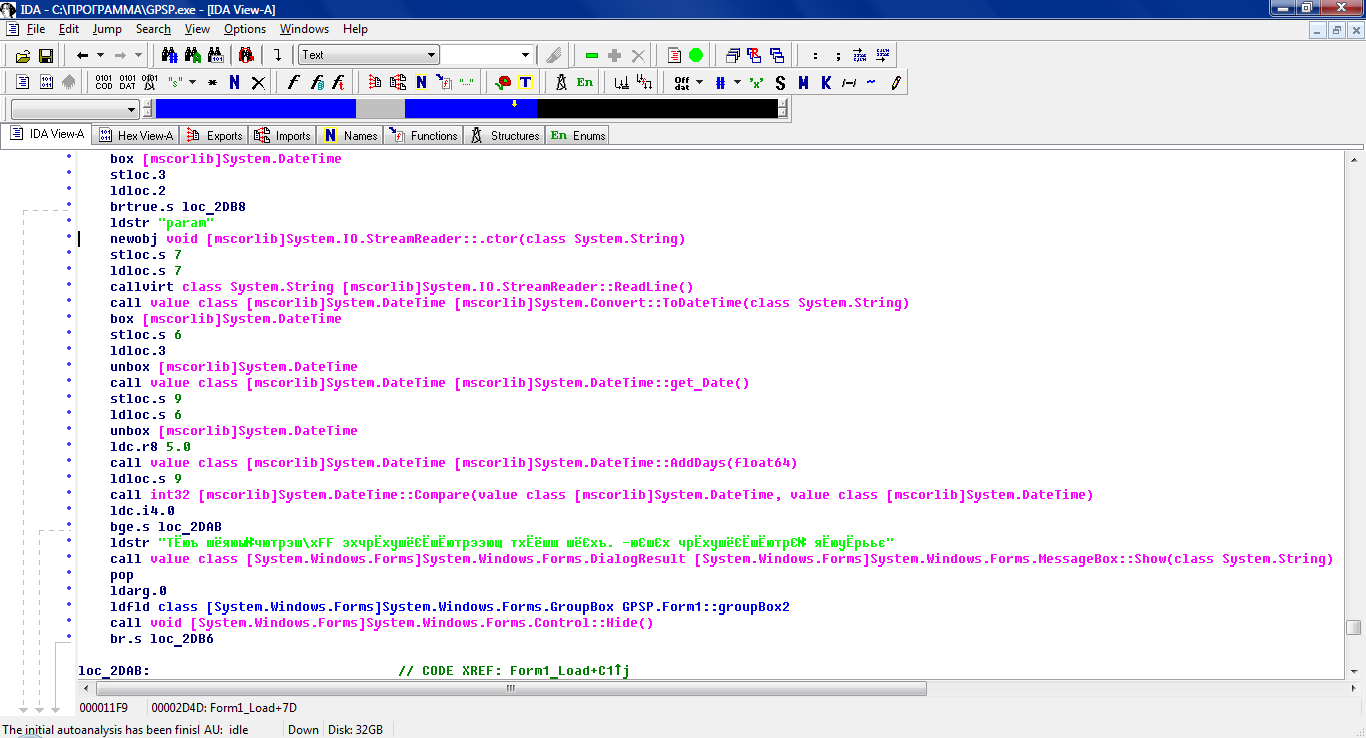
\includegraphics[width=\textwidth]{check_date}
  \caption{Функция проверки срока использования программы}
  \label{fig:6}
\end{figure}

На рисунке~\ref{fig:6} отмечено считывание даты установки из файла
\texttt{param}, а также срок равный 5 дням и функция сравнения
дат. Данные сведения могут быть использованы при попытках модификации
даты установки, либо при модификации программы.

\subsection{Анализ защиты с использованием монитора процессов}

Далее была проанализированы обращения программы к ресурсам файловой
системы и реестра при запуске и проверке регистрации, с помощью
программы \textit{ProcessMonitor}. На рисунке~\ref{fig:7} представлено
считывание признака регистрации из ключа реестра при запуске.

\begin{figure}[h!]
  \centering
  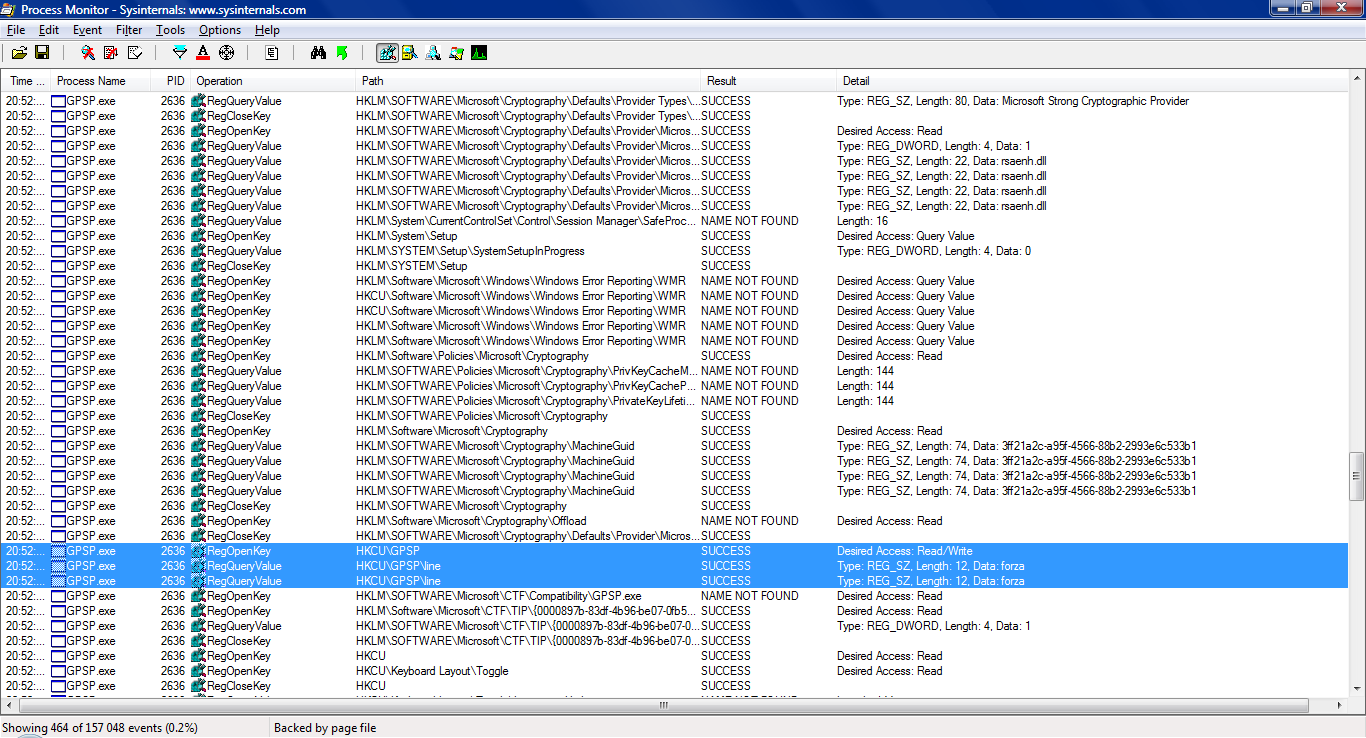
\includegraphics[width=\textwidth]{process}
  \caption{Обращения к реестру для проверки признака регистрации}
  \label{fig:7}
\end{figure}

Из полученных сведений можно построить алгоритм работы механизма
проверки регистрации. Кроме того, можно установить содержимое ключа
регистрации программы (строка-признак регистрации \texttt{forza}
отображается как содержимое ключа). Данные сведения могут быть
использованы при создании признака регистрации несанкционированным
способом.

\subsection{Анализ защиты с использованием отладчика}

В ходе исследования средствами отладчика выявлен условный переход,
управляющий проверкой регистрации. На рисунке~\ref{fig:8} на него
установлена точка останова.

\begin{figure}[h!]
  \centering
  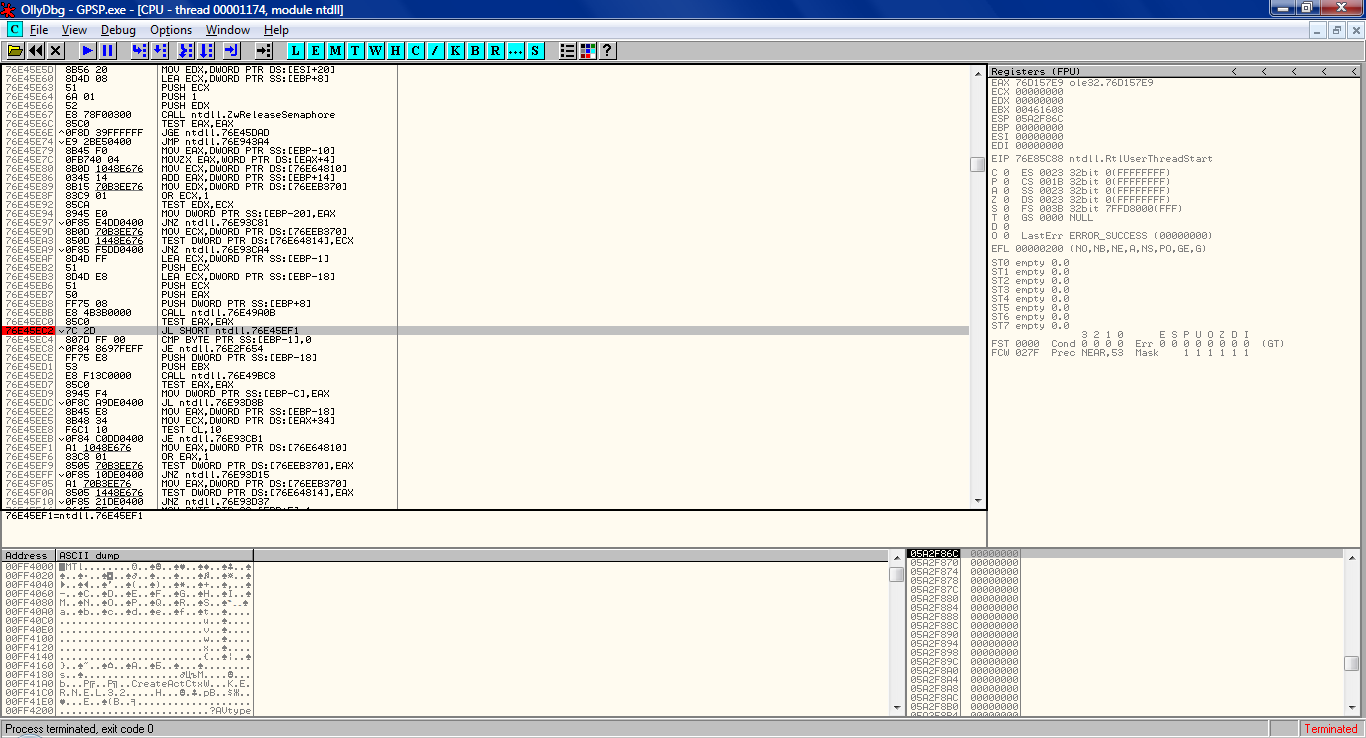
\includegraphics[width=\textwidth]{olly}
  \caption{Условный переход, управляющий проверкой регистрации}
  \label{fig:8}
\end{figure}

Модификация данного условного перехода средствами отладчика (например,
отключение проверки заменой перехода на команду NOP) приведет к снятию
защиты программы (результаты проверки не будут обрабатываться для
управления загрузкой программы).

В ходе исследования были выявлены уязвимости, позволяющие обойти
защиту программы: возможность изучения механизмов регистрации и
проверки регистрации, незащищенное хранение признака регистрации,
возможность модификации программы с целью отключения защиты.

Для повышения защиты программы следует ввести следующие усиления~\cite{4}:
\vspace{-5mm}
\begin{itemize}
\item разделение признака регистрации на несколько файлов и их
  шифрование с использованием данных даты установки, для вычисления
  ключа;
\item использование самомодифицирующегося кода: шифрование \linebreak
  критических участков программы и расшифровка их
  непосредственно в память процесса;
\item использование средств защиты от отладки;
\item защита файла, хранящего дату установки с использованием
  шифрования;
\item усложнения алгоритма работы программы с помощью ложных ветвей
  алгоритма и функций, не влияющих на работу программы;
\item отказ от использования осмысленных имен функций и использование
  функций переходников.
\end{itemize}

\cleardoublepage


%%% Local Variables: 
%%% mode: latex
%%% TeX-master: "../TermWork_PASIOB"
%%% End: 
